% objects.tex
%
% written 2022 by Werner Lemberg <wl@gnu.org>


% This file contains graphics used for the 'FreeType Design' documentation,
% part 2, 'Public Objects and Classes', and part 3, 'Internal Objects and
% Classes'.


% Here is one possibility to convert this LaTeX file to both PNG and SVG
% formats.
%
%   xelatex objects.tex
%
%   pdftoppm -png -f 1 -l 2 -r 120 objects.pdf objects
%   optipng objects-*.png
%
%   for i in 1 2; do
%     pdf2svg objects.pdf objects-$i.svg $i
%   done


\documentclass[tikz,
               svgnames, % for xcolor
               border=3mm]{standalone}

\usepackage{libertinus}

\usetikzlibrary{
  arrows.meta,
  calc,
  positioning
}


% Node styles.
\tikzset{
%
  % For normal lines.
  line/.style={
    line width=1pt},
%
  % For thin lines.
  thin line/.style={
    line width=0.5pt},
%
  % For the relation 'A has B'.
  has/.style={
    thin line,
    {Kite[length=12pt,
          width=6pt,
          inset=4pt]}-},
%
  % For the relation 'a child of A has B'.
  child has/.style={
    thin line,
    {Kite[open,
          length=12pt,
          width=6pt,
          inset=4pt]}-},
%
  % For boxes in general.
  box/.style={
    line,
    draw,
    inner xsep=5mm,
    inner ysep=3mm},
%
  % For boxes in the legend.
  legend box/.style={
    thin line,
    draw}
}


%%%%%%%%%%%%%%%%%%%%%%%%%%%%%%%%%%%%%%%%%%%%%%%%%%%%%%%%%%%%%%%%%%%%%%%%%%%%%

\begin{document}

% Basic object relationship.

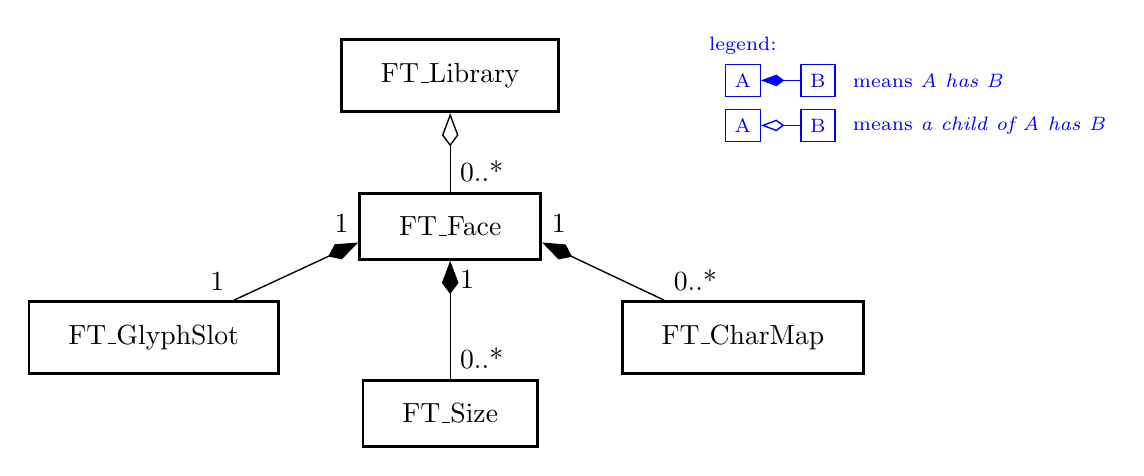
\begin{tikzpicture}
  \node[box] (F) {FT\_Face};
  \node[box] (L) [above=1cm of F] {FT\_Library};
  \node[box] (G) [below left=0.5cm and 1cm of F]{FT\_GlyphSlot};
  \node[box] (S) [below=1.5cm of F] {FT\_Size};
  \node[box] (C) [below right=0.5cm and 1cm of F]{FT\_CharMap};

  \draw[child has] (L) -- (F)
    node[above right, at end] {0..*};
  \draw[has] (F.190) -- (G)
    node[above left, at start] {1}
    node[above left, at end] {1};
  \draw[has] (F) -- (S)
    node[below right, at start] {1}
    node[above right, at end] {0..*};
  \draw[has] (F.-10) -- (C)
    node[above right, at start] {1}
    node[above right, at end] {0..*};

  \begin{scope}[blue,
                font=\scriptsize,
                arrows={[scale=0.7]}]
    \node[anchor=north west,
          above=3cm of C] (L) {legend:};

    \node[legend box,
          below=0mm of L] (A1) {A};
    \node[legend box,
          right=0.5cm of A1,
          label={right:\ means \textit{A has B}}] (B1) {B};
    \draw[has] (A1) -- (B1);

    \node[legend box,
          below=1ex of A1] (A2) {A};
    \node[legend box,
          right=0.5cm of A2,
          label={right:\ means \textit{a child of A has B}}] (B2) {B};
    \draw[child has] (A2) -- (B2);
  \end{scope}
\end{tikzpicture}


% Detailed object relationship.

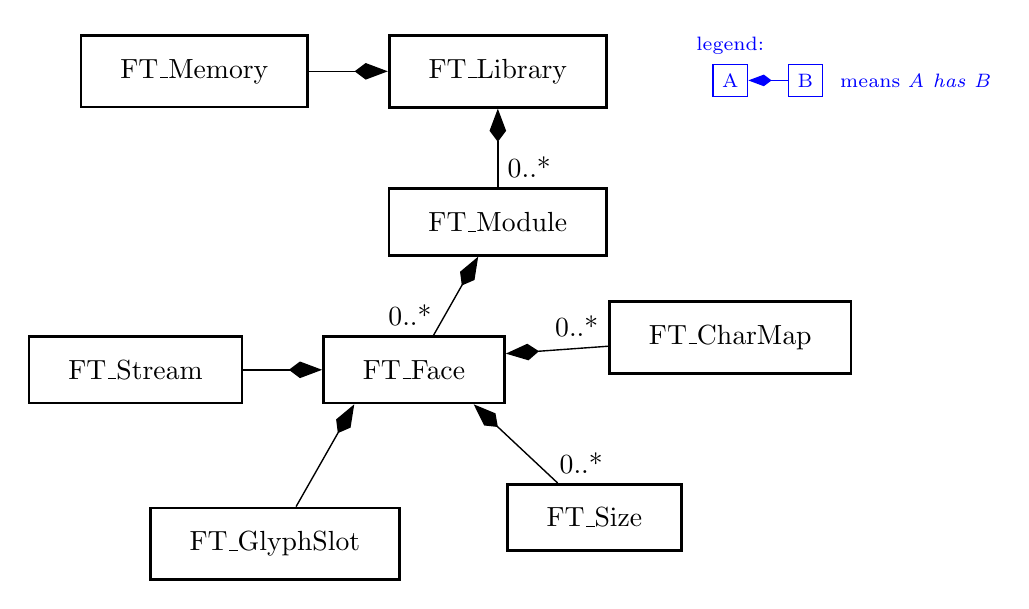
\begin{tikzpicture}
  \node[box] (F) {FT\_Face};
  \node[box] (M) [above right=1cm and -1.5cm of F] {FT\_Module};
  \node[box] (L) [above=1cm of M] {FT\_Library};
  \node[box] (Mem) [left=1cm of L] {FT\_Memory};
  \node[box] (Str) [left=1cm of F] {FT\_Stream};
  \node[box] (G) [below left=1.3cm and -1cm of F]{FT\_GlyphSlot};
  \node[box] (S) [below right=1cm and 0cm of F] {FT\_Size};
  \node[box] (C) [above right=-0.5cm and 1.3cm of F]{FT\_CharMap};

  \draw[has] (L) -- (Mem);
  \draw[has] (L) -- (M)
    node[above right, at end] {0..*};
  \draw[has] (M) -- (F)
    node[above left=0mm and -1mm, at end] {0..*};
  \draw[has] (F) -- (Str);
  \draw[has] (F.210) -- (G);
  \draw[has] (F.-30) -- (S)
    node[above right=0mm and -1mm, at end] {0..*};
  \draw[has] (F.10) -- (C)
    node[above left, at end] {0..*};

  \begin{scope}[blue,
                font=\scriptsize,
                arrows={[scale=0.7]}]
    \node[anchor=north west,
          above=3cm of C] (L) {legend:};

    \node[legend box,
          below=0mm of L] (A1) {A};
    \node[legend box,
          right=0.5cm of A1,
          label={right:\ means \textit{A has B}}] (B1) {B};
    \draw[has] (A1) -- (B1);
  \end{scope}
\end{tikzpicture}

\end{document}
